\chapter[Project Plan]{Project Plan}

\section{Project Aims}
The aim of this project is to evaluate the potential of integrating a Prolog-based optimization framework within the GraalVM compiler. Logic programming languages have demonstrated significant advantages in the program analysis phase of compilers. This project seeks to explore their application in the optimization phase—a complex and critical component of the compiler. Enhancing the optimization phase could lead to substantial improvements in program speed and performance.

\textbf{Aims}
\begin{compactitem}
    \item \textbf{Develop Prolog-Based Optimization Rules:} Implement Prolog rules for various optimization techniques within the Ahead-of-Time (AOT) compiler.
    \item \textbf{Integrate Prolog-Based Optimization:} Assess the feasibility of incorporating a Prolog-based optimization framework within the GraalVM compiler.
    \item \textbf{Enhance Optimization Expressiveness:} Evaluate how Prolog can improve the expressiveness and effectiveness of compiler optimizations compared to existing GraalVM techniques.
    \item \textbf{Evaluate New Optimizations:} Investigate potential new optimizations enabled by Prolog specifications and compare their performance against existing GraalVM optimization methods.
\end{compactitem}

\setcounter{secnumdepth}{3}

\section{Methodology}

\subsection{Prolog-Based Optimization Framework}
The Prolog-based optimization framework is composed of three key components. 

\textbf{Prolog fact generator:} Generate Prolog facts that accurately represent the IR graph of the program. This component will parse the IR and convert it into a Prolog-compatible format, allowing Prolog rules to operate on the program's structure. The approach involves traversing the IR graph and generating Prolog facts based on the graph's nodes and edges.

\textbf{Prolog optimization rules:} Express optimization rules as Prolog facts and predicates. This involves translating optimization concepts into Prolog syntax, ensuring that the rules are both expressive and applicable to the GraalVM compiler's intermediate representation (IR).

\textbf{Prolog-based optimizer:} Recursively querying Prolog optimization rules, executing Prolog queries, and applying transformations to the IR. This system should iteratively refine the program based on the query results. The component will be developed in Java and could potentially leverage the GNU Prolog for Java library to facilitate the execution of Prolog queries within the Java environment. 

To ensure compatibility between Prolog facts and rules, the development of the first two components will occur in parallel.

\subsection{Integration Into GraalVM Compiler}
After developing the standalone components of the Prolog-based optimizer, the next step is to integrate it with the GraalVM compiler. GraalVM is a substantially large and very complex project. Therefore, this integration may encounter potential compatibility issues. It is necessary to treat the integration phase as a distinct part of the development process. This involves modifying the GraalVM compiler to interface effectively with the Prolog-based optimizer and ensuring that the compiler can pass IR data to the Prolog-based optimizer and receive optimized IR data back for further processing.

\subsection{Testing}
Since the optimization phases involve significant transformations to the original code, ensuring the soundness and correctness of the optimizer is crucial. To achieve this, a comprehensive test suite is developed to:
\begin{compactitem}
    \item \textbf{Verify Prolog Rules:} Test the Prolog rules to ensure they function correctly and identify all valid optimization opportunities without introducing errors.
    \item \textbf{Validate Fact Generation:} Confirm that the generated Prolog facts accurately represent the original Intermediate Representation (IR), ensuring consistency and correctness.
    \item \textbf{Assess Integration:} Evaluate the integration of the Prolog-based optimizer with the GraalVM compiler, ensuring that the optimized code accurately reflects the original code and that no errors are introduced during the optimization process.
\end{compactitem}

\subsection{Evaluation}
After validating the optimizer's correctness, performance must be evaluated and compared with existing methods to determine any improvements offered by Prolog-based optimizations. Additionally, it is important to assess whether the declarative syntax enhances documentation, comprehension, and maintenance of the optimizer.
\begin{compactitem}
    \item \textbf{Performance Metrics:} Measure various performance metrics including execution speed, resource utilization (e.g., memory and CPU), and optimization throughput. Compare these metrics with those of existing GraalVM optimization techniques to gauge improvements or regressions.
    \item \textbf{Strengths and Weaknesses:} Identify and document the strengths and weaknesses of the Prolog-based optimizer. This analysis will help in understanding how well Prolog-based optimizations perform relative to traditional methods and where improvements can be made.
    \item \textbf{Potential New Optimizations:} Explore and document potential new optimization techniques that can be enabled by Prolog specifications. This involves identifying unique optimization opportunities that Prolog's declarative nature may unlock, which are not feasible with traditional imperative methods. 
\end{compactitem}

\newpage

\section{Timeline}
The project timeline is divided into two parts: the first half (Semester 2, 2024) and the second half (Semester 1, 2025). The timeline is further divided into 4 phases: Project Proposal, Proof of Concept, Extension and Evaluation, and Report and Demonstration. The total duration of the project is 30 weeks, with a commitment of 10 working hours per week. The first half involves conducting research, writing the project proposal, and developing a proof of concept. The second half focuses on refining and expanding the project to encompass a comprehensive set of optimization rules, as well as preparing the final paper, report, and presentation. The timeline may be adjusted based on the results of the proof of concept phase to accommodate unforeseen challenges or to incorporate additional development needs.  The distribution of weeks per task is illustrated in the timeline graph below.

\begin{figure}[h]
    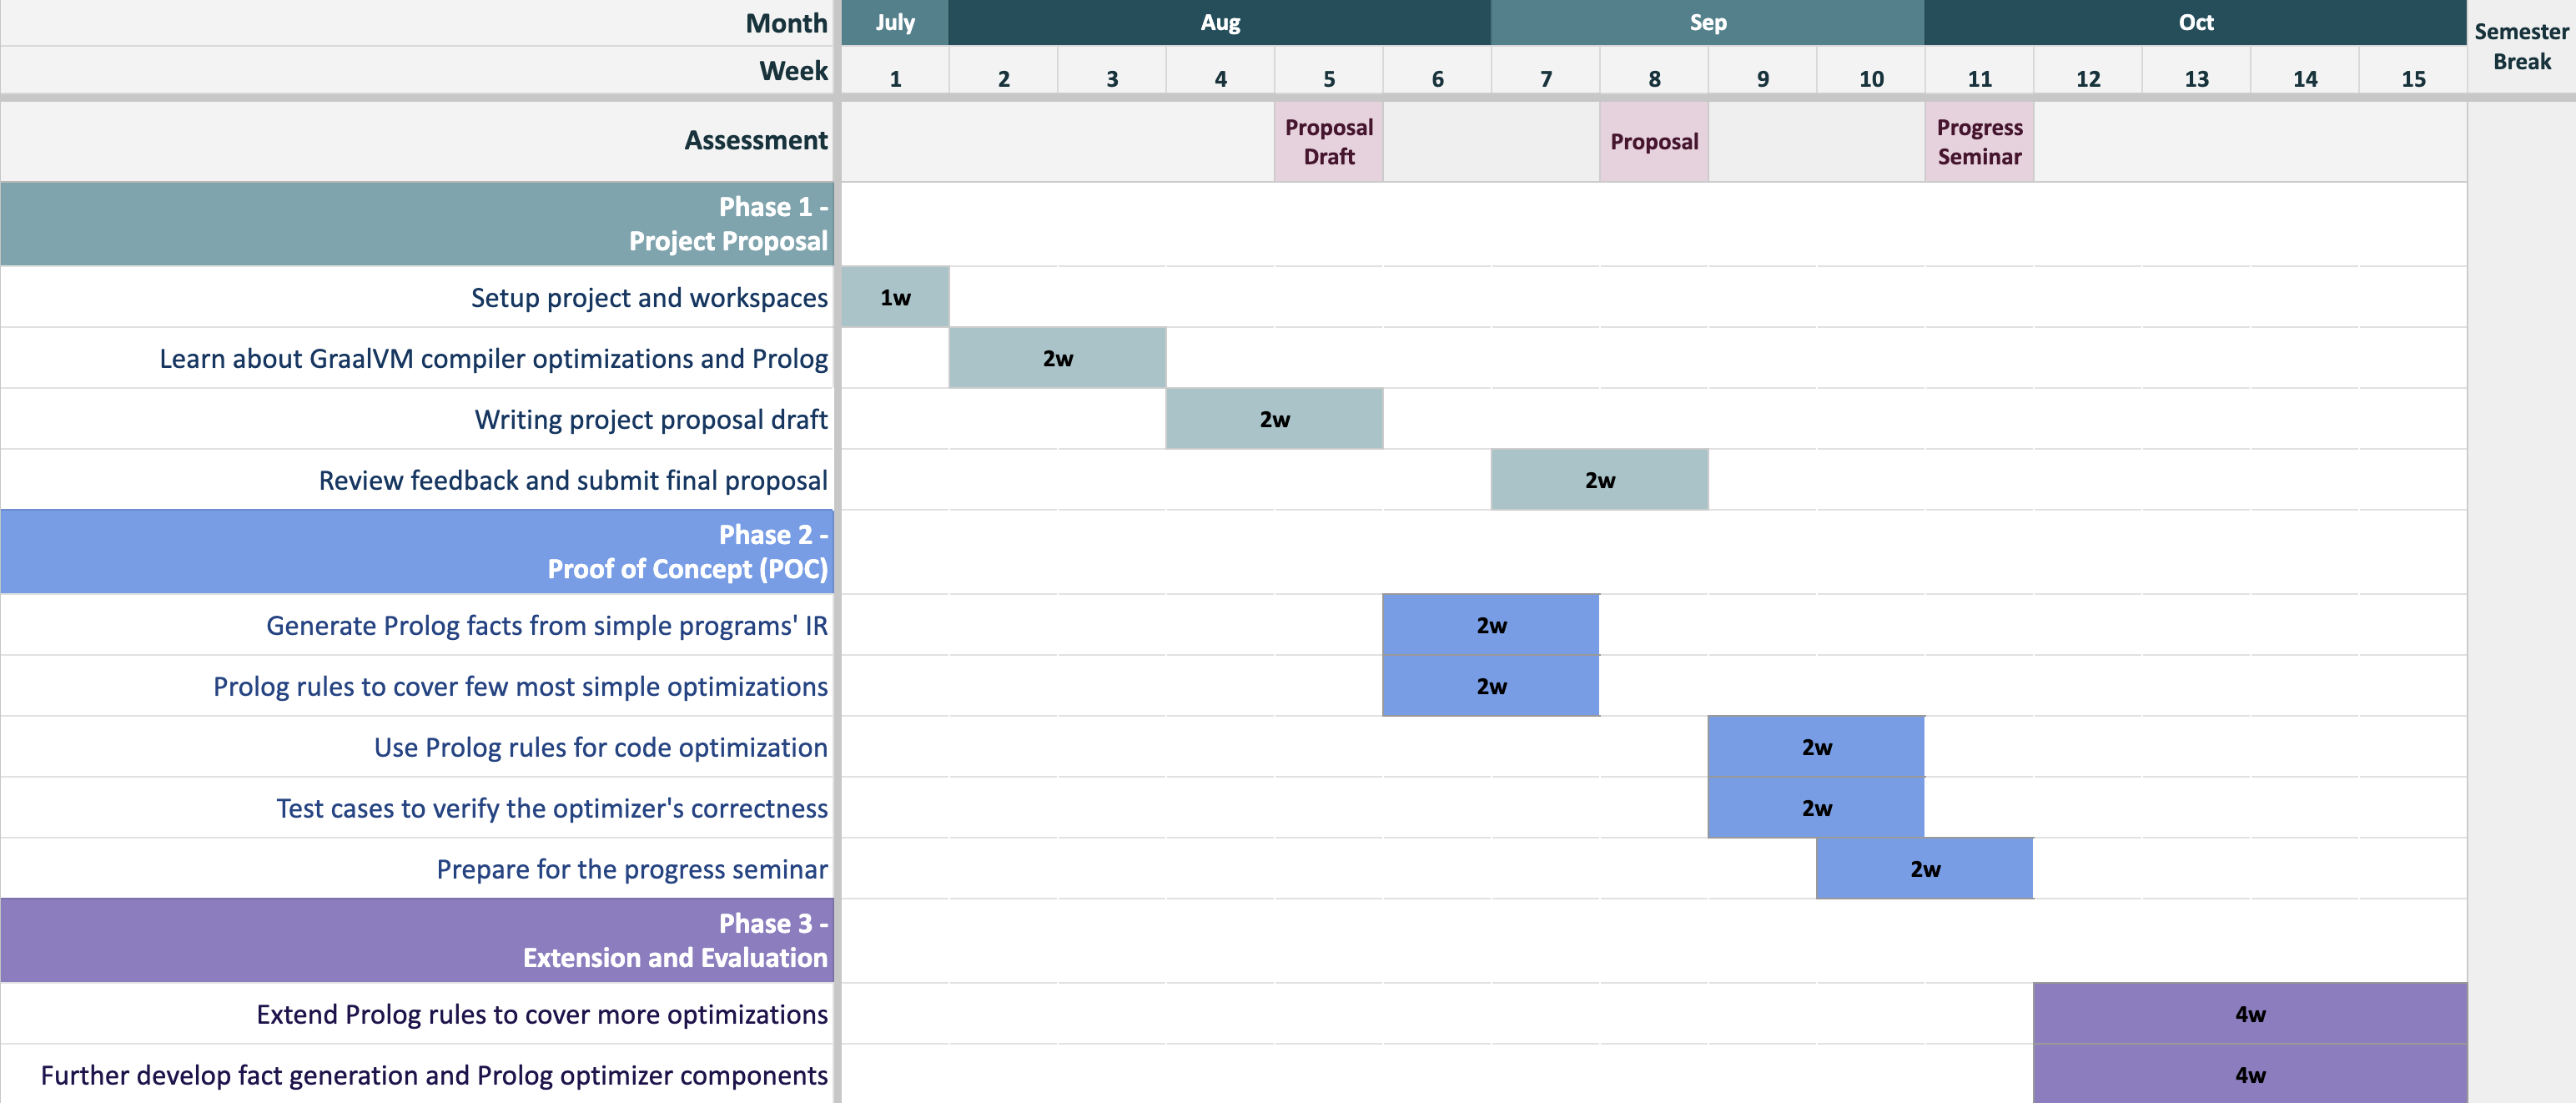
\includegraphics[width=1\textwidth]{Packages/PartA.png}
    \caption{Project Timeline (first half)}
\end{figure}
\begin{figure}[h]
    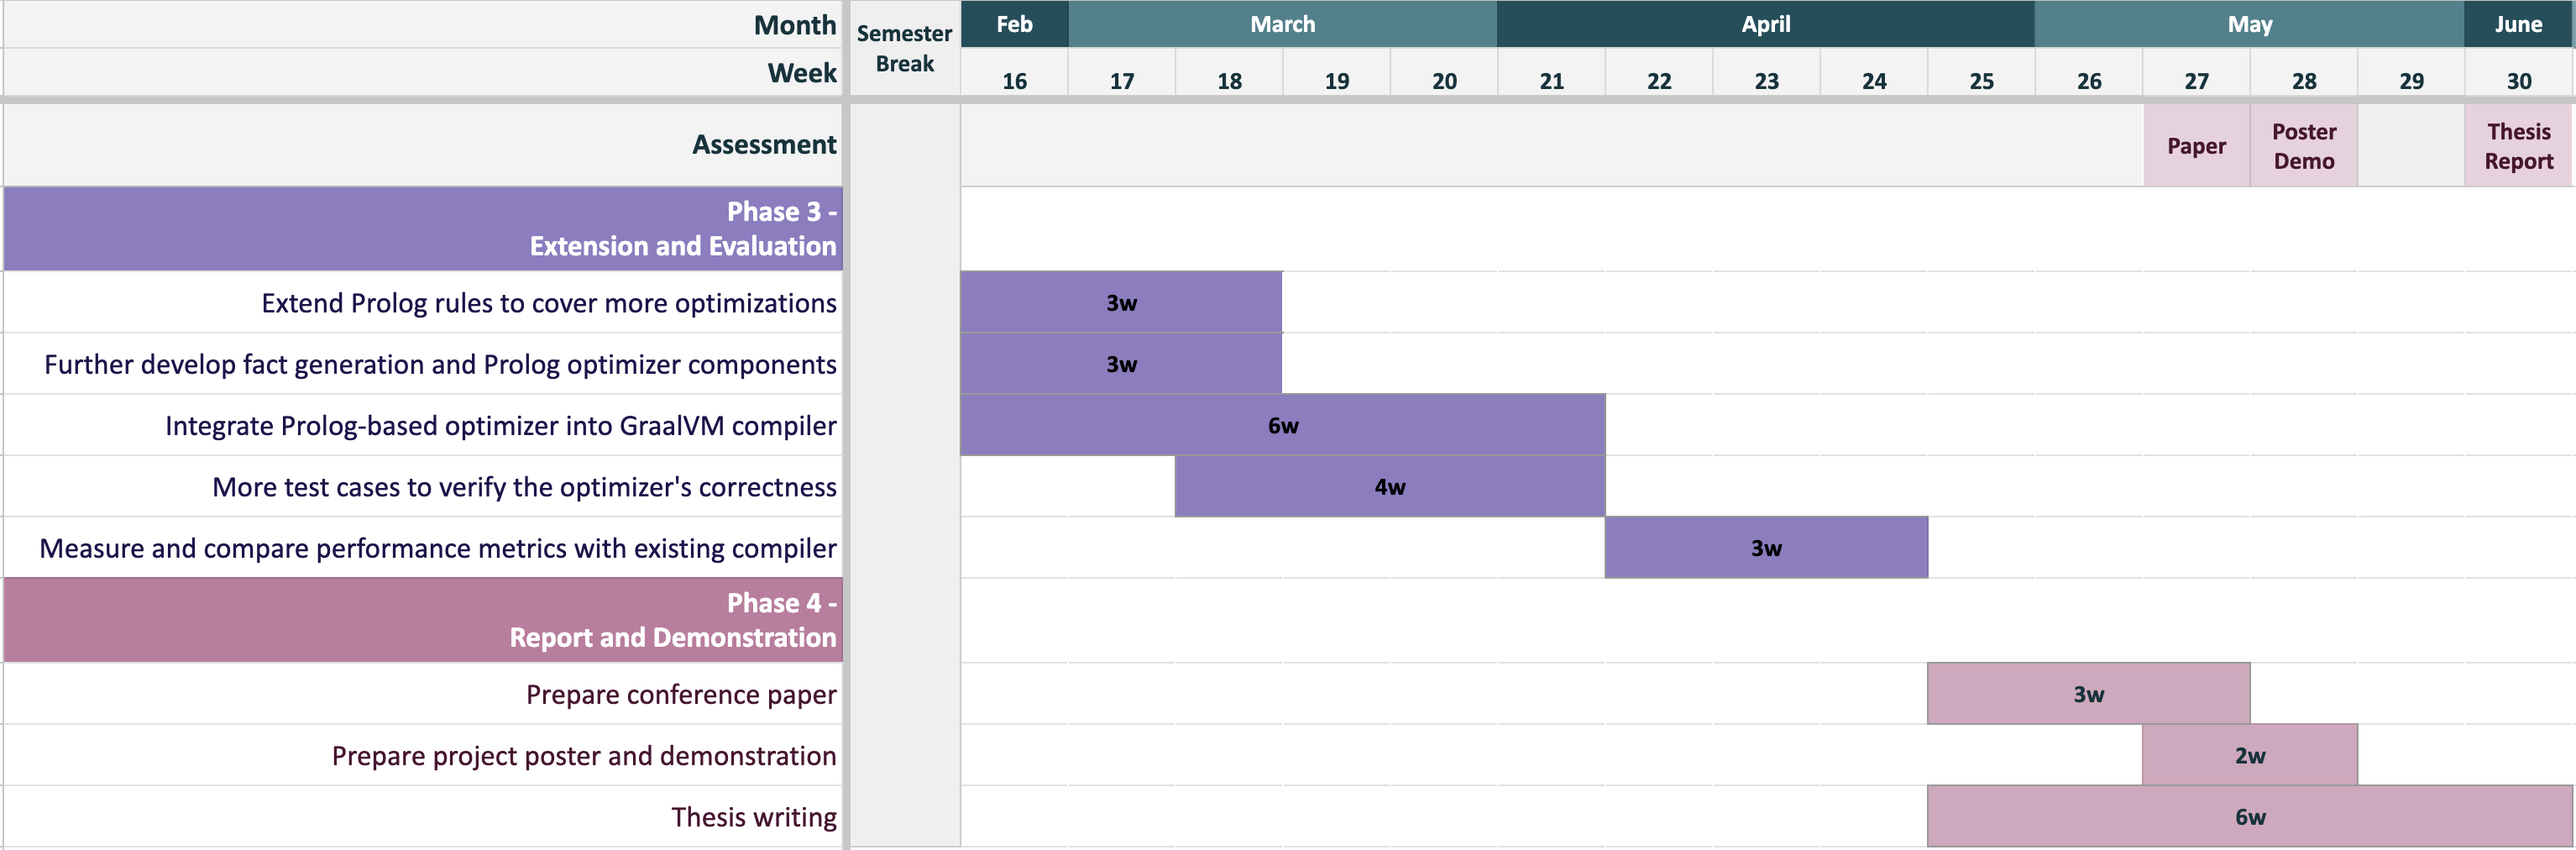
\includegraphics[width=1\textwidth]{Packages/PartB.png}
    \caption{Project Timeline (second half)}
\end{figure}

\newpage
Each project phase concludes with a milestone, except for the Extension and Evaluation phase, which includes two milestones due to a three-month semester break dividing this phase. The first three milestones occur during the first part of the project involve planning, validating the concept, and the initial development cycle. The final two milestones, scheduled for the second part, focus on advancing development and completing the final thesis.

\subsection{Milestone 1: Project Proposal}
\textbf{Date:} 19/09/2024 (Week 8) \\
\textbf{Deliveries:} Project proposal

To deliver the project proposal, several tasks need to be completed. The first week of the project involved meeting with the supervisors to gain a better understanding of the project and setting up the necessary tools and workspaces. The following two weeks focused on studying GraalVM compiler optimizations, intermediate representations (IR), and Prolog. The subsequent two weeks were dedicated to conducting additional research and a literature review in preparation for the draft proposal. Based on the feedback received, the final project proposal is expected to be delivered by the eighth week as an assessment item.

\subsection{Milestone 2: Proof of Concept (PoC) and Progress Seminar}

\textbf{Date:} 08/10/2024 (Week 11) \\
\textbf{Deliveries:} PoC and progress update presentation

In the second phase of the project, the focus will be on developing a proof of concept (PoC) for the Prolog-based optimizer. This PoC will employ a limited set of simple optimization techniques to assess the feasibility of the proposed approach. The PoC will also identify any additional development efforts required that may have been overlooked in the initial phase. Finally, this phase will conclude with a progress update seminar which is the second assessment item.

\subsection{Milestone 3: Initial Extension and Improvement Cycle}

\textbf{Date:} 01/11/2024 (Week 15) \\
\textbf{Deliveries:} More comprehensive set of optimization rules and a better Prolog-based optimizer

In the third phase, the focus will shift to extending and refining the proof of concept (PoC). Following the initial verification of optimization rules, efforts will be directed toward expanding the Prolog optimization rule sets to support more complex and advanced optimizations. Additionally, components such as the Prolog fact generator and the Prolog-based optimizer, will be revised and enhanced for increased robustness and efficiency, incorporating insights gained from the PoC results. The phase will conclude at the end of the semester, with a more comprehensive set of optimization rules and an improved optimizer from the previous phase.

\subsection{Milestone 4: Completion of Development and Testing}

\textbf{Date:} 25/04/2025 (Week 24) \\
\textbf{Deliveries:} Final version of the Prolog-based optimizer

The second half of the project will focus on continuing and enhancing the Prolog-based optimizer based on insights from the previous phase. A key objective will be to integrate the Prolog-based optimizer with the GraalVM compiler. This phase will also involve developing comprehensive test cases to ensure the optimizer’s correctness and robustness. Performance metrics will be assessed and compared with those of the existing GraalVM compiler to identify strengths and weaknesses. The phase will conclude with the finalization of the Prolog-based optimizer and a detailed review of its capabilities, performance, and potential for future enhancements.

\subsection{Milestone 5: Thesis Writing and Demonstration}
\textbf{Date:} 09/06/2025 (Week 30) \\
\textbf{Deliveries:} Final thesis report

With all development and testing completed in the previous phase, the final phase of the project will focus on preparing the conference paper, project poster, project presentation, and final thesis report, which are the remaining assessment items. The submission of the final thesis report will mark the project's completion.

\newpage

\section{Ethics \& Risk Assessment}
\subsection{Ethics Assessment}
This project exclusively engages with software and does not involve the collection or use of data from human or animal subjects. As a result, it does not require any substantial ethical considerations.
\subsection{Risk Assessment}
The table below outlines potential risks that could impact project success, along with corresponding mitigation strategies to minimize their likelihood and severity.
\renewcommand{\arraystretch}{1.3}
\begin{table}[h]
    \begin{tabularx}{1\textwidth} { 
        | >{\raggedright\arraybackslash}p{8em}
        | >{\raggedright\arraybackslash}p{4.5em} 
        | >{\raggedright\arraybackslash}p{4.5em} 
        | >{\raggedright\arraybackslash}p{3.5em} 
        | >{\raggedright\arraybackslash}X 
        | 
        }   
        \hline
        \textbf{Risk} & 
        \textbf{Likelihood} & 
        \textbf{Severity} & 
        \textbf{Risk Level} &
        \textbf{Mitigation Strategy}
        \\ 
        \hline
        Unable to meet key requirements and lagging behind scheduled milestones.
        & Possible & Significant & High & 
        Conduct regular meetings with supervisors and team members to assess project progress, identify and resolve any obstacles or difficulties, and ensure efficient time management.
        \\ 
        \hline
        Loss development progress due to computer problem.
        & Unlikely & Significant & Medium & 
        Backup all work progress to multiple places, e.g. code to GitHub and reports to drive.
        \\ 
        \hline
        Insufficient expertise in logical programming languages and the GraalVM compiler.
        & Likely & Minor & Medium &
        Dedicate time to acquiring domain knowledge and studying Prolog, GraalVM optimizations, and intermediate representation (IR) constructs. Consult supervisors regularly for guidance and support.
        \\ 
        \hline
        The Prolog-based optimizer may be less accurate and add performance overhead.
        & Possible & Moderate & Medium &
        Develop various test cases, conduct benchmarking to assess optimizer performance, and analyze the accuracy of the results.
        \\ 
        \hline
        Health issues while working with the project.
        & Possible & Moderate & Medium &
        Ensure that the project is systematically organized and well paced to prevent overwork and mitigate stress.
        \\ 
        \hline
        Safety issues in the workplace.
        & Unlikely & Minor & Low &
        Safety concerns are limited, given that the work is conducted in a controlled, in-house environment and involves only computer systems.
        \\ 
        \hline
    \end{tabularx}
\caption{Risk Assessment.}
\end{table}

